\documentclass{beamer}


\usetheme{Berlin}
\usefonttheme[onlylarge]{structurebold}
\setbeamerfont*{frametitle}{size=\normalsize,series=\bfseries}
\setbeamertemplate{navigation symbols}{}
\setbeamertemplate{caption}[numbered]

% Standard packages

\usepackage[english]{babel}
\usepackage[utf8]{inputenc}
\usepackage{times}
\usepackage[T1]{fontenc}
\usepackage{amsmath, amssymb}
\usepackage{multimedia}
\usepackage{caption}
\usepackage{tabularx}
\usepackage{changepage}

% Setup TikZ

\usepackage{tikz}
\usetikzlibrary{arrows}
\tikzstyle{block}=[draw opacity=0.7,line width=1.4cm]

% New useful definitions:

\newbox\mytempbox
\newdimen\mytempdimen

\newcommand\includegraphicscopyright[3][]{%
  \leavevmode\vbox{\vskip10pt\raggedright\setbox\mytempbox=\hbox{\includegraphics[#1]{#2}}%
    \mytempdimen=\wd\mytempbox\box\mytempbox\par\vskip1pt%
    \fontsize{3.5}{4}\selectfont{\color{black!25}{\vbox{\hsize=\mytempdimen#3}}}\vskip3pt%
}}

% Author, Title, etc.

\title[Time Pressure as Video Game Design Element and Basic Need Satisfaction] 
{%
  Time Pressure as Video Game Design Element and Basic Need Satisfaction%
}

\author[İrem Gökçe Yıldırım]
{
  İrem~Gökçe~Yıldırım
}

\institute[METU]
{
  Middle East Technical University
  \and
  \vskip+2mm
  \textit{iremgokceyildirim@gmail.com}
}

%\author[Author, Another] % (optional, use only with lots of authors)
%{F.~Author\inst{1} \and S.~Another\inst{2}}
% - Give the names in the same order as the appear in the paper.
% - Use the \inst{?} command only if the authors have different
%   affiliation.
%
%\institute[Universities of Somewhere and Elsewhere] % (optional, but mostly needed)
%{
%  \inst{1}%
%  Department of\emph{ Computer Science\\
%  University of Somewhere
%  \and
%  \inst{2}%
%  Department of Theoretical Philosophy\\
%  University of Elsewhere}
%% - Use the \inst command only if there are several affiliations.
%% - Keep it simple, no one is interested in your street address.}


\date[August 2015]
{August 12, 2015}


% The main document

\begin{document}

\begin{frame}
  \titlepage
\end{frame}

\begin{frame}{Outline}
  \tableofcontents[hideothersubsections]
\end{frame}


\section{Introduction}

\subsection{Motivation}
\begin{frame}{Why we continue popping bubbles, \dots,  till 3 AM in the morning?}

\includegraphicscopyright [width=1.0\textwidth,clip]{images/Figure_1_candycrush}
{ \textit{Candy Crush Is So Addictive That This Man Didn't Notice He Tore A Tendon},\\ Retrieved from \url{ http://www.huffingtonpost.com/2015/04/14/tendon-tear-candy-crush_n_7062942.html}}
\label {fig:candycrush}

\end{frame}

\begin{frame}{Reasons Behind Gaming}
	Players play games for "FUN" \cite{Kocca2013WhitePaper}
	\begin{block}{Enjoyment Models and Engagement Factors}
    \begin{itemize}
    \item Mechanics/Dynamics/Aesthetics (MDA) \cite{hunicke2004mda}
    \item Achievement/Social/Immersion \cite{yee2007motivations}
    \item GameFlow \cite{Sweetser2005flow}     
    \item \dots 
    
    \end{itemize}
  \end{block}
  \begin{block}{Psychological Approach}
    \begin{itemize}
    \item \alert{Self-Determination Theory (SDT)} \cite{RyanDeci2000IntrinsicExtrinsic} : Power of SDT
    \end{itemize}
  \end{block}
\end{frame}

\begin{frame}{Motivational Pull of Video Games (SDT Approach)}
	\begin{block}{Underlying Motivational Factors}
    \begin{itemize}
    \item Basic Psychological Need Satisfaction
    	\begin{itemize}
    		\item \alert{Autonomy}: \textcolor{green!50!black}{being in control and acting volitional}
  			\item \alert{Competence} : \textcolor{green!50!black}{self-efficacy and mastery}
  			\item \alert{Relatedness} : \textcolor{green!50!black}{meaningful connection to others}
  		\end{itemize}
  	 \item Player Experience of Need Satisfaction (PENS) \cite{PrzybylskiRigbyRyan2006MotivationPullofGames}
    \item Motivational Outcomes (Intrinsic Motivation, Enjoyment, Well-being, etc.)
    \end{itemize}
    \end{block}
\end{frame}

\subsection{Contribution}

\begin{frame}{Contribution of the Study}
    \begin{itemize}
    \item Motivation through game design elements
    \item Specific game element contribution to the corresponding need satisfactions
    \item Relationship with other outcomes (Flow, Engagement, Performance and Enjoyment)
     \item Utilizing game elements to make better games
    \end{itemize}
\end{frame}



\subsection{Hypotheses}

\begin{frame}{Presented Work}
\textbf{Aim:} To reveal the relationship between time pressure and basic need satisfaction and consequences.

\begin{figure}[h]
\centering
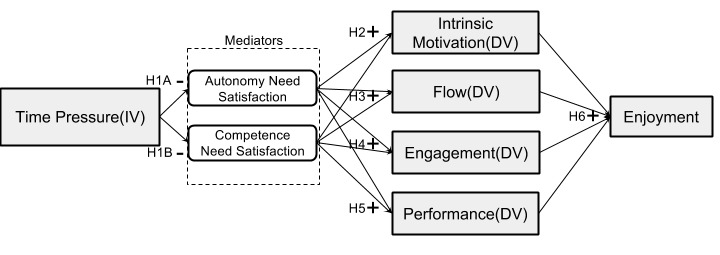
\includegraphics [width=\textwidth,clip]{images/Figure_2_Framework}
\caption[hypotheses]{Proposed Research Framework}
\label {fig:hypotheses}
\end{figure}

\end{frame}

\section{Background and Related Work}

\subsection{Self-Determination Theory}
\begin{frame}{Self-Determination Theory}
Well-formulated framework of self-initiated and autonomous actions \cite{RyanDeci2000IntrinsicExtrinsic}
\begin{itemize}
  \item \alert{Intrinsic Motivation}:  intrinsic appeal of the activity itself, based on one's own interest
  \begin{itemize}
  	\item no external pressure, rewards, punishment or introjected controls (avoiding guilt or anxiety)
  \end{itemize}
  \item \alert{Basic Psychological Needs}
  	 \begin{itemize}
  		\item Autonomy : \textcolor{green!50!black}{choices, informative rewards}
  		\item Competence : \textcolor{green!50!black}{mastering skills, optimal challenges, achievement goals, positive performance feedbacks}
  		\item Relatedness : \textcolor{green!50!black}{sharing, caring, feeling secure}
  	\end{itemize}
  \end{itemize}
 
\end{frame}


\subsection{Video Games and Basic Psychological Needs}
\begin{frame}{Basic Need Satisfaction in Games}
Readily availability of games, consistency between expectations and outcomes in games and intensive exposition of all three needs are some key characteristics of motivational power of video games \cite{RyanRigby2011glued}
\begin{itemize}
\item \alert{Autonomy in Games}:  flexibility over movement and strategies, choices over tasks, character customization
  \item \alert{Competence in Games}: new abilities, progressive challenges, performance feedbacks, heroic narrative and intuitive controls
  \item \alert{Relatedness in Games}: cooperative and competitive group play, teammate interactions (healing), social network integration 
   \end{itemize}
\end{frame}

\begin{frame}{Related Work}
 \vspace{-1em}
\includegraphicscopyright [width=1\textwidth, height=.85\textheight, clip]{images/Figure_3_RelatedWorks.jpg}
{Studies Manipulating Some Game Elements for Motivational Accordances \cite{Peng2012NeedSupportiveFeatures}, \cite{Baldwin2014DynamicDifficulty}, \cite{Schmierbach2014DifficultyMotivation}, \cite{Mekler2013PointsLevesLeaderboards}, \cite{Tamborini2010definemedia}, \cite{Dennie2012AutonomyMotivation}}
\label {fig:candycrush}
\end{frame}

\subsection{Time Pressure and Basic Psychological Need Satisfaction}
\begin{frame}{Time Pressure and Autonomy and Competence}
\textbf{Time Pressure} : one of the ten ingredients of great games (as cited in \cite{Deterding2011Gamification})
\begin{itemize}
	\item \textbf{H1A}: \alert{Time pressure will diminish Autonomy} in the  experimental condition
		\begin{itemize}
			\item feeling of being under control \cite{RyanDeci2000bSDT, RyanDeci2000IntrinsicExtrinsic, Radel2013NeedRestoration, hattie2007powerofFeedback} (as cited in \cite{Deci2000GoalPursuit, PrzybylskiRigbyRyan2006MotivationPullofGames})
			\item absence of choices
			\item reduction of decision time
		\end{itemize}
  \item \textbf{H1B}: \alert{Time pressure will diminish Competence} in the experimental condition
  \begin{itemize}
  		\item time limit is a challenge itself \cite{adams2013fundamentals, schell2014art, teh2013can, BlohmL2013Gamification}
		\item using skills ineffectively with shortened decision making \cite{romero2013time}
		\item decrease in self-efficacy with failures
	\end{itemize}
   \end{itemize}
\end{frame}

\subsection{Time Pressure and Consequences}
\begin{frame}{Time Pressure and Outcomes}
\begin{itemize}
	\item \textbf{H2}: \alert{Time pressure will diminish Intrinsic Motivation} in the  experimental condition
		\begin{itemize}
			\item direct relation with autonomy and competence need satisfaction \cite{PrzybylskiRigbyRyan2006MotivationPullofGames}
			\item mediating effects of autonomy and competence \cite{PrzybylskiRigbyRyan2006MotivationPullofGames, Tamborini2010definemedia,Schmierbach2014DifficultyMotivation}
			\item deadlines have undermining effects on intrinsic motivation \cite{amabile1976timePressure, Sheldon2008Manipulating, Deci2000GoalPursuit}
		\end{itemize}
  \item \textbf{H3}: \alert{Time pressure will diminish Flow} in the  experimental condition
  \begin{itemize}
  		\item having control over actions (autonomy)
		\item time limit as a challenge should be balanced with skills (competence) \cite{romero2013time, Tavassolian2011TimeBalancing}
		\item mediating effects of autonomy and competence
	\end{itemize}
   \end{itemize}
\end{frame}

\begin{frame}{Time Pressure and Outcomes}
\begin{itemize}
	\item \textbf{H4}: \alert{Time pressure will diminish Engagement} in the  experimental condition
		\begin{itemize}
			\item shorter time limits leads disengagement \cite{Lomas2013ChallengeOptimization}
			\item decrease in self-interest and self-efficacy
			\item mediating effects of autonomy and competence
		\end{itemize}
  \item \textbf{H5}: \alert{Time pressure will diminish Performance} in the  experimental condition
  \begin{itemize}
  		\item decisions made under time pressure apt to be wrong \cite{Linehan2009TimeDecisionMaking, Amabile2002Creativity, romero2013time}
  		\item making effective strategies is very hard under time pressure \cite{Locke1996ComplexGoalTime}
		\item as time limit gets shorter, players’ performance decreases (number of failures increases) \cite{Lomas2013ChallengeOptimization}
		\item positive correlation between competence and performance \cite{McEwan2012ControlDevice, Sheldon2008Manipulating}
	\end{itemize}
   \end{itemize}
\end{frame}

\begin{frame}{Time Pressure and Outcomes}
\begin{itemize}
	\item \textbf{H6}: \alert{Time pressure will diminish overall Enjoyment} in the  experimental condition
  		\begin{itemize}
  			\item Intrinsic Motivation \cite{PrzybylskiRigbyRyan2006MotivationPullofGames}, Flow \cite{Sweetser2005flow}, Engagement \cite{boyle2012engagement} and Performance \cite{trepte2011pleasures, klimmt2009player} are associated with enjoyment
		\end{itemize}
   \end{itemize}
\end{frame}

\section{Method}

\subsection{Participants}
\begin{frame}{Participants}
\begin{itemize}
	\item 69 male ; 37 female
	\item Undergraduates and graduate students from METU
	\item from Psychology Department and Informatics Institute graduate programs
\end{itemize}
\end{frame}

\subsection{Measures}
\begin{frame}{Measures}
Accessed through \href {https://www.surveymonkey.com}{SurveyMonkey}, 7-point Likert scale
\begin{enumerate}
\item Demographics and Game Play Questionnaire {\tiny[\hyperlink{appB1}{AppendixB}]}
\item \alert{Manipulation Check Scale} {\tiny(Time Limit Realization, Perceived Time Pressure and Task Difficulty) [\hyperlink{appC}{AppendixC}]}
\item \alert{PENS Scale} {\tiny[\hyperlink{appD}{AppendixD}]}
	\begin{itemize}
		\item In-Game Autonomy ($\alpha = .85$)
		\item In-Game Competence ($\alpha = .80$)
	\end{itemize}
\item \alert{Intrinsic Motivation Inventory} (IMI) ($\alpha = .82$) {\tiny [\hyperlink{appE}{AppendixE}]}
\item \alert{GameFlow Scale} ($\alpha = .86$) {\tiny [\hyperlink{appF}{AppendixF}]}
\item \alert{Engagement Scale} ($\alpha = .76$) {\tiny [\hyperlink{appG}{AppendixG}]}
\item \alert{Game Play Data} (for Performance) {\tiny [\hyperlink{appH}{AppendixH}]}

\end{enumerate}
\end{frame}

\subsection{Procedure}
\begin{frame}{Procedure}
\alert{Two stages}: 
\begin{enumerate}
\item Pre-Questionnaire (Demographics and Game Play Questionnaire)
\item Lab Session
	\begin{enumerate}
		\item Game Play session at the Lab, \textasciitilde 2 min.
		\item Post-Questionnaire at the Lab (Scales), \textasciitilde 10 min.
	\end{enumerate}
\end{enumerate}
%target game and demo
\end{frame}

\begin{frame}{The Experiment}
\alert{The Experiment}: 
\begin{itemize}
\item Between Subject Experiment
\item 2 Conditions: Control (Time Limit OFF) and Experimental Group (Time Limit ON, 120 sec.)
\end{itemize}
\alert{Target Game}: 
\begin{itemize}
\item 3D Shooter (“Survival Shooter" by Unity Technologies)
\begin{itemize}
	\item Not well-known (data gathering issues) but highly ranked in the Asset Store (to engage in 2 min.)
\end{itemize}
\item audio-visually immersive, not complex, intuitively controlled
\item open-world kind (ensuring different game completion times)

\end{itemize}
\end{frame}

\begin{frame}{Target Game}
\alert{Target Game}: Tutorial part - Training Part - GamePlay
\begin{center}
\movie[poster, showcontrols]%, externalviewer] 
  {
\includegraphics[width=.7\textwidth, height=.7\textheight]{images/Placeholder.png}}{images/Demo_Cutted.mov}
\end{center} 
\end{frame}

\begin{frame}{Target Game and Basic Need Satisfaction}
\alert{Autonomy Supportive Elements}
\begin{itemize}
\item freedom (open-world kind)
\item make your own decisions (choose whichever dolls to kill)
\item strategy (choose how to kill the dolls)
\item meaningful narrative
\end{itemize}
\alert{Competence Supportive Elements}
\begin{itemize}
\item audio-visual performance feedback (granular - taking damage and cumulative - health bar, left dolls number)
\item intuitive controls
\item optimal challenge
	\begin{itemize}
		\item the amount of damages of both the players and the dolls
		\item obstacle rich environment
	\end{itemize}		
\end{itemize}  
\end{frame}


\section{Results}

\subsection{Preliminary Analysis}
\begin{frame}{Manipulation Check}

\begin{table}[h]
\captionsetup{labelfont=bf, justification=justified,singlelinecheck=false}
\caption[T-Test Results for Manipulation Check]{T-Test Results for Manipulation Check}
\label {table:manipulationcheck}
\fontsize{8pt}{8}\selectfont
{\renewcommand{\arraystretch}{1.5}
\begin{tabularx}{1.0\textwidth}{lccl}
\hline
\multicolumn{1}{c}{} & \begin{tabular}[c]{@{}c@{}}Control Group \\ ($n$=50)\end{tabular} & \begin{tabular}[c]{@{}c@{}}Experimental Group\\ ($n$=51)\end{tabular} &  \\ \hline
\multicolumn{1}{c}{Time Press. Manipulation Scale} & \multicolumn{2}{c}{$M$ ($SD$)} & $t$(99) \\ \hline
Realization of time limit & 2.64 (2.02) & 5.45 (1.72) & 7.53* \\
Perceived time pressure & 2.29 (1.62) & 4.39 (2.07) & 5.65*** \\
Perceived task difficulty & 2.30 (1.61) & 2.96 (1.95) & 1.86 \\ \hline
*$p$ \textless .05, ***$p$ \textless .001 & \multicolumn{1}{l}{} & \multicolumn{1}{l}{} & \multicolumn{1}{l}{}
\end{tabularx}}
\end{table}

\end{frame}

\subsection{Primary Analysis}
\begin{frame}{Primary Analysis}

\begin{table}[h]
\captionsetup{labelfont=bf, justification=justified,singlelinecheck=false}
\caption[T-Test Results for Dependent Variables]{T-Test Results for Dependent Variables}
\label {table:primaryresults}
\fontsize{8pt}{8}\selectfont
{\renewcommand{\arraystretch}{1.2}
\begin{tabularx}{1.0\textwidth}{lccl}
\hline
\multicolumn{1}{c}{} & \begin{tabular}[c]{@{}c@{}}Control Group \\ ($n$=50)\end{tabular} & \begin{tabular}[c]{@{}c@{}}Experimental Group\\ ($n$=51)\end{tabular} &   \\ \hline
\multicolumn{1}{c}{Dependent variables} & \multicolumn{2}{c}{$M$ ($SD$)} & $t$ (99) \\ \hline
Autonomy & 3.03 (1.31) & 3.37 (1.36) & 1.24 \\
Competence & 4.83 (1.56) & 4.86 (1.40) & 0.11\\
Intrinsic Motivation & 3.82 (0.88) & 3.96 (0.90) & 0.76 \\
Flow & 4.84 (1.44) & 5.38 (1.02) & 2.21* \\
Engagement & 3.52 (0.88) & 3.81 (0.95) & 1.62 \\
Performance (Left Health / 100) & 92.7 (17.4) & 94.5 (11.3) & 0.62 \\
Enjoyment & 4.83 (1.41) & 4.94 (1.01) & 0.46 \\
Game Play Spent Time (in sec) & 130.62 (39.4) & 110.49 (10.9) & 3.51** \\ \hline
*$p$ \textless .05, **$p$ \textless .01 & \multicolumn{1}{l}{} & \multicolumn{1}{l}{} & \multicolumn{1}{l}{}
\end{tabularx}}
\end{table} 

\end{frame}

\begin{frame}{Subgroups Emerged in the Experimental Groups}

\begin{table}[H]
\captionsetup{labelfont=bf, justification=justified,singlelinecheck=false}
\caption[Frequencies of Game End Conditions in the Target Game of the Experiment]{Frequencies of Game End Conditions in the Target Game of the Experiment}
\label {table:gameendconditions}
\begin{tabular}{lcc}
\hline
\multicolumn{1}{c}{} & \begin{tabular}[c]{@{}c@{}}Control Group \\ ($n$=53)\end{tabular} & \begin{tabular}[c]{@{}c@{}}Experimental Group \\ ($n$=53)\end{tabular} \\ \hline
\multicolumn{1}{c}{Game End Conditions} & \multicolumn{2}{c}{$n$} \\ \hline
Successful & 50 & 29 \\
No Health  & 3 & 2 \\
No Time & - & 22 \\ \hline
\end{tabular}
\end{table}

\end{frame}

\begin{frame}{Comparison of Subgroups in the Experimental Groups}
\begin{adjustwidth}{-1.5em}{-1.5em}
\begin{table}[h]
\captionsetup{labelfont=bf, justification=justified,singlelinecheck=false,skip=0pt,belowskip=8pt}
\caption[One-Way ANOVA Results for Dependent Variables between No Time and Successful Subgroups in Control and Experimental Conditions]{\fontsize{9pt}{8}\selectfont One-Way ANOVA Results for Dependent Variables between No Time and Successful Subgroups in Control and Experimental Conditions}
\label {table:anovaresults}
\fontsize{8pt}{8}\selectfont
{\renewcommand{\arraystretch}{1.2}
\begin{tabular}{lcccccl}
\hline
 & \begin{tabular}[c]{@{}c@{}}Control Group \\ ($n$ = 53)\end{tabular} &  & \multicolumn{2}{c}{\begin{tabular}[c]{@{}c@{}}Experimental Group \\ ($n$ = 53)\end{tabular}} & \multicolumn{1}{l}{} & \multicolumn{1}{l}{} \\ \cline{2-2} \cline{4-5}
 & \begin{tabular}[c]{@{}c@{}}Successful \\ ($n$ = 50)\end{tabular} &  & \begin{tabular}[c]{@{}c@{}}Successful \\ ($n$ = 29)\end{tabular} & \begin{tabular}[c]{@{}c@{}}No Time \\ ($n$ = 22)\end{tabular} & \multicolumn{1}{l}{} & \multicolumn{1}{l}{} \\ \cline{2-5}
\multicolumn{1}{c}{} & \multicolumn{4}{c}{$M$} & $F$ (2,98) & Sig. \\ \hline
Perceived Time Press. & 2.29 &  & 3.76 & 5.23 & 21.4 & .000*** \\
Autonomy & 3.03 &  & 3.20 & 3.56 & 1.23 & .30 \\
Competence & 4.83 &  & 5.23 & 4.38 & 2.16 & .12 \\
Intrinsic Motivation & 3.82 &  & 3.83 & 4.12 & 0.96 & .39 \\
Flow & 4.84 &  & 5.14 & 5.69 & 3.70 & .028* \\
Engagement & 3.52 &  & 3.60 & 4.10 & 3.24 & .043* \\
Performance & 92.7 &  & 98.1 & 89.8 & 2.31 & .11 \\ 
Enjoyment & 4.83 &  & 4.93 & 4.97 & .11 & .89 \\ \hline
*$p$ \textless .05, ***$p$ \textless .001 & \multicolumn{1}{l}{} & \multicolumn{1}{l}{} & \multicolumn{1}{l}{} & \multicolumn{1}{l}{} & \multicolumn{1}{l}{} & \multicolumn{1}{l}{}
\end{tabular}}
\end{table}

\end{adjustwidth}
\end{frame}

\begin{frame}{Comparison of Subgroups in the Experimental Groups} 
\begin{figure}[h]
\centering
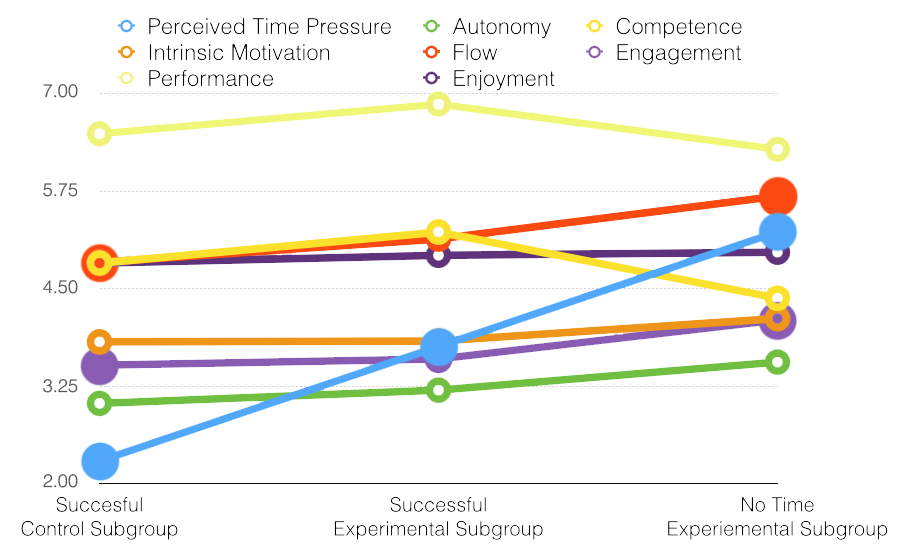
\includegraphics [width=.8\textwidth,clip]{images/Figure_4_Results}
\captionsetup{labelfont=bf, justification=justified,singlelinecheck=false,skip=0pt,belowskip=0pt}
\caption[meanscores]{\fontsize{6.5pt}{6.5}\selectfont Mean Scores of the Dependent Variables for Subgroups in the Experimental Conditions. \it {Note: Performance results are scaled to the range 0-7 from 0-100. Significantly different variables are represented as dots.}}
\label {fig:meanscores}
\end{figure}
\end{frame}

\subsection{Discussion}
\begin{frame}{Discussion}
\begin{enumerate}
\item Players experienced more \alert{Flow} and \alert{Engagement} \textbf{even though they failed} in the game because of time limit
	\begin{itemize}
	\item Zeigarnik effect
	\end{itemize}
\item \alert{Competence} and \alert{Performance} (Left Health/100) approached significance between \textbf{no time and successful experimental subgroups}, ($p$ = .10, $p$ = .11, respectively)
	\begin{itemize}
		\item increases with time limit; however, if perceived time pressure increases under that time limit, it starts to diminish them
		\item Zeigarnik effect (for the increase), drop in self-efficacy and failures in achieving the goal in the given time limit (for the decrease)
	\end{itemize}
\end{enumerate}
\end{frame}

\begin{frame}{Discussion Cont.}
\begin{figure}[h]
\centering
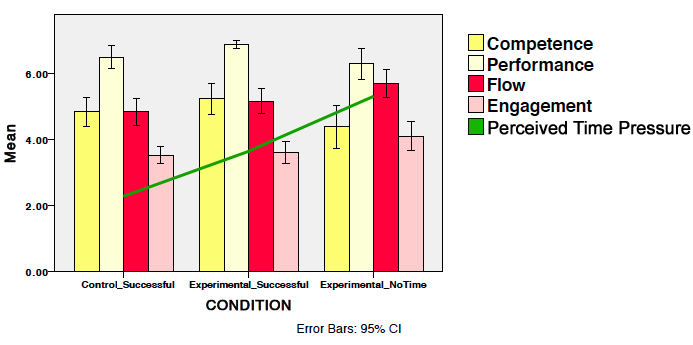
\includegraphics [width=.9\textwidth,clip]{images/Figure_5_Discussion}
\captionsetup{labelfont=bf, justification=justified,singlelinecheck=false,skip=0pt,belowskip=0pt}
\caption[meanscores]{\fontsize{6.5pt}{6.5}\selectfont Mean Scores of the Competence, Performance, Flow and Engagement for Subgroups in the Experimental Conditions}
\label {fig:discussion}
\end{figure}
\end{frame}

\begin{frame}{Discussion Cont.}
\begin{adjustwidth}{-1.5em}{-1.5em}
\begin{enumerate}\addtocounter{enumi}{1}
\item \alert{Competence} and \alert{Performance} approached significance
	\begin{itemize}
		\item \textbf{Inverted-U relationship} between competence (and performance) and time pressure as a challenge \cite{Lomas2013ChallengeOptimization}
		\begin{figure}[h]
\centering
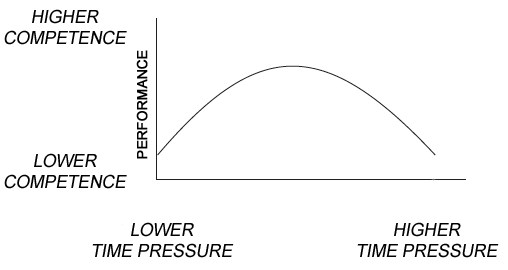
\includegraphics [width=.5\textwidth,clip]{images/Figure_6_Discussion2}
\captionsetup{labelfont=bf, justification=justified,singlelinecheck=false,skip=0pt,belowskip=0pt}
\caption[inverted]{\fontsize{6.5pt}{6.5}\selectfont Curvilinear Relationship Between Competence-Performance and Perceived Time Pressure}
\label {fig:discussion}
\end{figure}
	\end{itemize}
\item \textbf{Change} in \alert{autonomy} (increased) and \alert{competence} (decreased) \textbf{oppositely} in the experimental group as time pressure increased
\end{enumerate}
\end{adjustwidth}
\end{frame}

\section{Conclusion and Future Work}

\subsection{Conclusion}
\begin{frame}{General Limitations}

  \begin{enumerate}
  \item \textbf{Participants}
  	\begin{itemize}
  		\item Power of the study is low (\alert{more sample size})
  		\item With \alert{more game play experience} (6 of 100, hardcore gamers)
  		\item With \alert{wide distribution of age} (86 of 101, 20-26)
  		\item \alert{Experience with wide range of game genres} (17 of 101, platform; 27 of 101, puzzle games)
  	\end{itemize}
  \item \textbf{Game Genre Effect}
  	\begin{itemize}
  		\item Time limit in 3D shooter game is unusual
  		\item Mastering controls under time pressure
  	\end{itemize}
  \item \textbf{Other Supportive Game Elements}
  	\begin{itemize}
  		\item Isolated game features may not be very effective in facilitating motivation \cite{McNamara2010PointsFeedback}
  		\item No options, character customization, mastery on skills, recovery choices to support autonomy and competence
  	\end{itemize}
  \end{enumerate}
\end{frame}

\begin{frame}{Conclusion}
\begin{adjustwidth}{-1.5em}{-1.5em}
  \begin{enumerate}
  \item \alert{Contribution of a specific game design element} (time limit) to the motivational pull of video games
  \item Players’ \alert{flow and engagement increases with time pressure}
  	\begin{itemize}
  		\item Implementation of time limit in games (e.g. in quests) may increase immersion
  	\end{itemize}
  \item An \alert{indication of curvilinear relationship} between \textbf{time pressure} as a challenge and \textbf{competence and performance}
  \begin{itemize}
  	\item There may be an \textbf{intermediate level of perceived time pressure} (as a challenge) provided by time limit mechanics which results in \textbf{maximum competence and performance accompanied by flow and engagement}
  	\item \textbf{Positive outcomes} such as flow, engagement and performance may be \textbf{explained from the perspective of basic need satisfaction}
  	\end{itemize}
  \end{enumerate}
  \end{adjustwidth}
\end{frame}

\subsection{Future Work}
\begin{frame}{Future Work}
\begin{adjustwidth}{-1.8em}{-1.8em}
  \begin{enumerate}
  \item A \alert{factorial design} may be conducted to observe the effects of \alert{different time limits}
  \begin{itemize}
  	\item With an \textbf{optimal level of time pressure}, autonomy, competence and other outcomes may be facilitated.
  	\item \textbf{Additional scale items} to measure Zeigarnik and failure (and the need for replay triggered by this failure) effects on flow, engagement, performance and competence
  \end{itemize}
  \item A \alert{formulation of need satisfactions} for a wide range of \textbf{game genres} \cite{RyanRigby2011glued}, by a wide range of \textbf{individual game design elements}
  \item \alert{Interrelations between game design elements} to facilitate the need satisfactions (e.g. \textbf{time limit with achievements, mastering skills, scores, co-play})
  \item \alert{A design heuristics} as a guideline \textbf{based on psychological satisfaction} to make better games
  \end{enumerate}
 \end{adjustwidth}
\end{frame}

\section{References}
\begin{frame}[allowframebreaks]
\fontsize{5pt}{5}\selectfont
  \frametitle<presentation>{References}
\bibliography{references}
\bibliographystyle{abbrv}
\end{frame}


\appendix
\section*{Appendix}

\begin{frame}[label=appA, plain]{Appendix A}
  \begin{columns}[t]
    \column{1.0\textwidth}
    \begin{exampleblock}{Informed Consent Form}
      \tiny \textbf{Genel Bilgiler}
\\ \tiny Bu çalışma ODTÜ Enformatik Enstitüsü Oyun Teknolojileri Yüksek Lisans Programı öğrencilerinden İrem Gökçe Yıldırım tarafından yürütülmektedir. Bu form sizi araştırma koşulları hakkında bilgilendirmek icin hazırlanmıştır.
\\Bu calışmanın amacı bazı oyun tasarım özellikleri ve edinilen psikolojik deneyimlerin arasindaki ilişkileri incelemektir. Arastırma internet üzerinden doldurulacak bir anket, devamında tamamlanacak olan bir laboratuvar çalışmasını içermektedir. Anket yaklaşık 5 dakika, laboratuvar çalışması ise 15 dakika sürecektir.
\\Araştırmada yaklaşık 100 katılımcı hedeflenmektedir. Üniversite öğrencileri katılımcı olarak davet edilecek, çalışmaya katılanlar bu duyurunun yapildiği ders için bonus puan alacaklardir. Alinacak puan dersin oğretim üyesi tarafından belirlenecektir. 
\\ \tiny \textbf{Riskler ve Faydalar}
\\ \tiny Araştırma katılımcı için herhangi bir risk veya fayda içermemektedir.
\\ \tiny \textbf{Gönüllülük Esası}
\\ \tiny Bu çalışmaya katılmak tamamen gönüllülük esasına dayalıdır. Çalışmayı istediginiz zaman bırakabilir, çalışma esnasında cevap vermek istemediğiniz sorular olursa boş bırakabilirsiniz.
\\ \tiny \textbf{Gizlilik Esası}
\\ \tiny Çalismaya katılanlardan toplanan veriler tamamen gizli tutulacak, veriler ve kimlik bilgileri herhangi bir şekilde eşleştirilmeyecektir. Katılımcıların isimleri bağımsız bir listede toplanacaktır. Ayrıca toplanan verilere sadece araştırmacılar ulaşabilecektir. Bu araştırmanın sonuçları bilimsel ve profesyonel yayınlarda veya eğitim amaçlı kullanılabilir, fakat katılımcılarin kimliği gizli tutulacaktır.
\\ \tiny \textbf{Irtibat}
\\ \tiny Çalışmayla ilgili soru ve yorumlarınızı araştırmacıya gokce.aydin@metu.edu.tr adresinden iletebilirsiniz veya 543 342 4219`'lu telefondan İrem Gökçe Yıldırım`'a ulaşabilirsiniz.
\\ \tiny \textbf{Katılımcı Onayı}
\\ \tiny \textbf{*Yukarıdaki bilgileri okudum ve bu araştırmaya gönüllü olarak katiımayı kabul ediyorum.}
\\ \begin{math}
	\square \mbox{ Evet} ~~~
	\square \mbox{ Hayır}
	\end{math}
    \end{exampleblock}
  \end{columns}  
\end{frame}

\begin{frame}[label=appB1, plain]{Appendix B-1}
  \begin{columns}[t]
    \column{1.0\textwidth}
    \begin{exampleblock}{Demographics and Game Play Questionnaire}
    \fontsize{6pt}{7.2}\selectfont
      \begin{enumerate}
\item Yaşınız?
	\rule{5cm}{1pt}
\item Cinsiyetiniz?
	\begin{math}
	\square \mbox{ Kadın} 
	\square \mbox{ Erkek}
	\end{math}
\item Lisans Anadalı Fakülteniz?
	\begin{math}
	\bigcirc \mbox{ Mühendislik}
	\bigcirc \mbox{ Fen Bilimleri}
	\bigcirc \mbox{ Mimarlık}
	\bigcirc \mbox{ Eğitim}
	\bigcirc \mbox{ Sosyal Bilimler}
	\bigcirc \mbox{ İktisadi ve İdari Bilimler}
	\bigcirc \mbox{ Diğer (Lütfen Belirtiniz) }\rule{5cm}{1pt}
	\end{math}
\item Video oyunları oynar mısınız?
	\begin{math}
	\square \mbox{ Evet} 
	\square \mbox{ Hayır}
	\end{math}
\item *Haftada kaç saat video oyunları oynarsınız?
	\begin{math}
	\bigcirc \mbox{ 1 saatten az}
	\bigcirc \mbox{ 1-5}
	\bigcirc \mbox{ 5-10}
	\bigcirc \mbox{ 10-15}
	\bigcirc \mbox{ 15'den fazla}
	\end{math}
\item *Kaç senedir video oyunları oynuyorsunuz?
	\begin{math}
	\bigcirc \mbox{ 1'den az}
	\bigcirc \mbox{ 1-3}
	\bigcirc \mbox{ 3-5}
	\bigcirc \mbox{ 5-7}
	\bigcirc \mbox{ 7'den fazla}
	\end{math}
\item Hangi tip oyunları oynamaktan hoslanırsınız?(Çoklu seçim yapabilirsiniz.)
	\begin{math}
	\square \mbox{ Birinci Şahis Nişancı Oyunları (First Person Shooter)} \newline
	\square \mbox{ Rol Yapma Oyunları (Role Playing Games)} \newline
	\square \mbox{ Devasa Çok Oyunculu Çevrimici Rol Yapma Oyunları (MMORPG)} \newline
	\square \mbox{ Aksiyon Oyunları (Action Games)} \newline
	\square \mbox{ Macera Oyunları (Adventure Games)} \newline
	\square \mbox{ Puzzle Oyunları (Puzzle Games)} \newline
	\square \mbox{ Strateji Oyunları} \newline
	\square \mbox{ Gerçek Zamanlı Strateji Oyunları (Real Time Strategy Games)} \newline
	\square \mbox{ Sıra Tabanlı Strateji Oyunları (Turn Based Strategy Games)} \newline
	\square \mbox{ Gündelik Oyunlar (Casual Games)} \newline
	\square \mbox{ Platform Oyunları} \newline
	\square \mbox{ Spor Oyunları} \newline
	\square \mbox{ Simulasyonlar} \newline
	\square \mbox{ Diğer(Lütfen Belirtiniz) }\rule{5cm}{1pt}
	\end{math}
\end{enumerate}
    \end{exampleblock}
  \end{columns}  
\end{frame}

\begin{frame}[label=appB2, plain]{Appendix B-2}
  \begin{columns}[t]
    \column{1.0\textwidth}
    \begin{exampleblock}{Demographics and Game Play Questionnaire, cont.}
    \fontsize{6pt}{7.2}\selectfont
      \begin{enumerate}\addtocounter{enumi}{7}
\item Oyunlarda en çok hoşunuza giden özellikler nelerdir?(Çoklu seçim yapabilirsiniz.) \newline
	\begin{math}
	\square \mbox{ Arayüz} \newline
	\square \mbox{ Karakterler-Modeller} \newline
	\square \mbox{ Ses Efektleri-Müzik} \newline
	\square \mbox{ Stratejik Davranabilme} \newline
	\square \mbox{ Zaman Baskısı} \newline
	\square \mbox{ Oyun Mekaniği} \newline
	\square \mbox{ Hareket Kabiliyetleri ve Kontroller} \newline
	\square \mbox{ Çoklu Oyun Oynayabilme} \newline
	\square \mbox{ Hikaye} \newline
	\square \mbox{ Başarı ve Kazanımlar} \newline
	\square \mbox{ Avatar Özelleştirebilme} \newline
	\square \mbox{ Diğer(Lütfen Belirtiniz) }\rule{5cm}{1pt}
	\end{math}
\item Kullandıgınız oyun platformları nelerdir?(Çoklu seçim yapabilirsiniz.)
	\begin{math}
	\square \mbox{ PC}
	\square \mbox{ Xbox}
	\square \mbox{ PlayStation}
	\square \mbox{ PlayStation Portable}
	\square \mbox{ Wii}
	\square \mbox{ Android Mobil Cihazlar}
	\square \mbox{ iOS Mobil Cihazlar} \newline
	\square \mbox{ Diğer(Lütfen Belirtiniz) }\rule{5cm}{1pt}
	\end{math}
\item Kendinizi nasıl hedefi olan bir oyuncu olarak tanımlarsınız?
	\begin{math}
	\bigcirc \mbox{ Öğrenmeye ve yetkinliklerini arttırmaya çalışan} \newline
	\bigcirc \mbox{ Öğrenememekten ve yetkinliklerini arttıramamaktan endişe duyan} \newline
	\bigcirc \mbox{ Diğerlerinden daha iyi performans göstermeye çalışan} \newline
	\bigcirc \mbox{ Diğerlerinden kötü perfomans göstermekten kaçınan} \newline
	\end{math}
\end{enumerate}
    \end{exampleblock}
  \end{columns}  
\end{frame}

\begin{frame}[label=appC, plain]{Appendix C}
  \begin{columns}[t]
    \column{1.0\textwidth}
    \begin{exampleblock}{Manipulation Check Scale}
     \fontsize{6pt}{7.2}\selectfont
      Aşağıdaki her bir ifadenin sizin düşüncenize göre ne kadar doğru olduğunu, aşağıdaki ölçek skalasını kullanarak belirtiniz.\\

\hspace{1.5cm}\makebox[8cm][s]{1 2 3 4 5 6 7} \par
\hspace{1cm}\makebox[11cm][s]{\parbox[c]{3cm}{\centering Kesinlikle katılmıyorum} \parbox{2.7cm}{\centering Ne katılıyorum ne katılmıyorum} \parbox{3cm}{\centering Kesinlikle katılıyorum}} \\
\fontsize{8pt}{7.2}\selectfont
\begin{enumerate}
\item Oyundaki görseller guzeldi.
\item Oyunda kullanılan objeleri kolayca tanımlayabildim.
\item \alert{Oyunu oynarken zaman kısıtlamasi vardı.}
\item Oyunda kullanılan müzikler ve ses efektleri etkileyiciydi.
\item Oyunun kontrolleri öğrenmek oldukça kolaydı.
\item \alert{Oyunu oynarken zaman baskisi altındaydım.}
\item Oyunda ortamı gezip, objeleri incelemek istedim.
\item \alert{Oyunda hedef görevi gerçekleştirmek zordu.}
\item Bu oyunu oynamaya gelecekte devam edebilirim.
\item Oyun kontrolleri sezgiseldi.
\item Oyunda birşey yapmak istediğimde, karşılık gelen kontrolleri hatırlamak kolaydı.
\end{enumerate}
    \end{exampleblock}
  \end{columns}  
\end{frame}

\begin{frame}[label=appD, plain]{Appendix D}
  \begin{columns}[t]
    \column{1.0\textwidth}
    \begin{exampleblock}{PENS Scale}

\small \textbf{In-Game Autonomy Scale}
\begin{enumerate}
\item Oyun ilginç seçenek ve tercihler sunuyor.
\item Oyun ilginç seyler yapmanıza olanak sağlıyor.
\item Oyunda çok fazla özgürlük hissettim.
\end{enumerate}

\small \textbf{In-Game Competence Scale}
\begin{enumerate}
\item  Oyunda kendimi yeterli hissettim.
\item  Oynarken kendimi becerikli ve etkili hissettim.
\item  Oynama yeteneğim ile oyundaki mücadeleler çok dengeli bir sekilde örtüşüyordu.
\end{enumerate}

    \end{exampleblock}
  \end{columns}  
\end{frame}

\begin{frame}[label=appD1, plain]{Appendix D-1}
  \begin{columns}[t]
    \column{1.0\textwidth}
    \begin{exampleblock}{PENS Scale (Original) \cite{Dennie2012AutonomyMotivation, PrzybylskiRigbyRyan2006MotivationPullofGames, Peng2012NeedSupportiveFeatures}}

\small \textbf{In-Game Autonomy Scale}
\begin{enumerate}
\item The game provides me with interesting options and choices
\item The game lets you do interesting things
\item I experienced a lot of freedom in the game
\end{enumerate}

\small \textbf{In-Game Competence Scale}
\begin{enumerate}
\item  I feel competent at the game.
\item  I feel very capable and effective when playing.
\item  My ability to play the game is well matched with the game's challenges.
\end{enumerate}

    \end{exampleblock}
  \end{columns}  
\end{frame}

\begin{frame}[label=appE, plain]{Appendix E}
  \begin{columns}[t]
    \column{1.0\textwidth}
    \begin{exampleblock}{IMI Scale (Enjoyment and Intrinsic Motivation)}
     \fontsize{8pt}{7.2}\selectfont

\begin{enumerate}
\item \alert{Oyunu oynarken keyif aldım.} -Enjoyment
\item \alert{Oyunu oynamak eğlenceliydi.} -Enjoyment
\item \alert{Oyunun sıkıcı olduğunu düsünüyorum. (R)} -Enjoyment
\item \alert{Oyun dikkatimi toplayamadı. (R)} -Enjoyment
\item \alert{Oyunu oynamayı çok ilginç buldum.} -Enjoyment
\item \alert{Oyunu oynamanın oldukça keyifli olduğunu düşünüyorum.} -Enjoyment
\item \alert{Oyunu oynarken, oyundan ne kadar keyif aldığımı düşünüyordum.} -Enjoyment
\item Bu oyunda çok fazla efor sarfettim.
\item Oyunda çok fazla çabaladım.
\item Oyunda iyi yapabilmek benim için önemliydi.
\item Oynarken kendimi çok gergin hissettim.
\item Oynarken çok rahattım. (R)
\item Oynarken kendimi endişeli hissettim.
\item Oynarken üzerimde baskı hissettim.
\end{enumerate}

    \end{exampleblock}
  \end{columns}  
\end{frame}

\begin{frame}[label=appE1, plain]{Appendix E-1}
  \begin{columns}[t]
    \column{1.0\textwidth}
    \begin{exampleblock}{IMI Scale (Original) \href{http://www.selfdeterminationtheory.org/intrinsic-motivation-inventory/}{\tiny  [www.selfdeterminationtheory.org]}}
     \fontsize{8pt}{7.2}\selectfont

\textbf{Interest/Enjoyment}
\begin{enumerate}
\item \alert{I enjoyed doing this activity very much.}
\item \alert{This activity was fun to do.}
\item \alert{I thought this was a boring activity. (R)}
\item \alert{This activity did not hold my attention at all. (R)}
\item \alert{I would describe this activity as very interesting.}
\item \alert{I thought this activity was quite enjoyable.}
\item \alert{While I was doing this activity, I was thinking about how much I enjoyed it.}
\end{enumerate}

\textbf{Effort/Importance}
\begin{enumerate}\addtocounter{enumi}{7}
\item I put a lot of effort into this.
\item I tried very hard on this activity.
\item It was important to me to do well at this task.
\end{enumerate}

\textbf{Pressure/Tension}
\begin{enumerate}\addtocounter{enumi}{10}
\item I felt very tense while doing this activity.
\item I was very relaxed in doing these. (R)
\item I was anxious while working on this task.
\item I felt pressured while doing these.
\end{enumerate}

    \end{exampleblock}
  \end{columns}  
\end{frame}

\begin{frame}[label=appF, plain]{Appendix F}
     \fontsize{10pt}{10}\selectfont
  \begin{columns}[t]
    \column{1.0\textwidth}
    \begin{exampleblock}{GameFlow Scale (Immersion)}

\begin{enumerate}
\item Oynarken etrafımdakilerin daha az farkındaydım.
\item Oynarken daha az farkındalık sahibiydim ve günlük yaşam hakkında daha az kaygılıydım.
\item Oynarken değiştirilmiş bir zaman deneyimi yaşadım.
\item Kendimi duygusal olarak oyunun içindeymişim gibi hissettim.
\item Tüm duyularımla kendimi oyunun içindeymişim gibi hissettim.
\end{enumerate}

    \end{exampleblock}
  \end{columns}  
\end{frame}

\begin{frame}[label=appF1, plain]{Appendix F-1}
     \fontsize{10pt}{10}\selectfont
  \begin{columns}[t]
    \column{1.0\textwidth}
    \begin{exampleblock}{GameFlow Scale (Immersion) (Original) \cite{Sweetser2005flow}}

\begin{enumerate}
\item Players should become less aware of their surroundings
\item Players should become less self-aware and less worried
about everyday life or self
\item Players should experience an altered sense of time
\item Players should feel emotionally involved in the game
\item Players should feel viscerally involved in the game
\end{enumerate}
\end{exampleblock}

\begin{exampleblock}{EGameFlow Scale (Immersion) (Original) \cite{Fu2009EGameFlow}}
\begin{enumerate}
\item I become unaware of my surroundings while playing the game
\item I temporarily forget worries about everyday life while playing the game
\item I experience an altered sense of time
\item I feel emotionally involved in the game
\item I feel viscerally involved in the game
\end{enumerate}
\end{exampleblock}
  \end{columns}  
\end{frame}


\begin{frame}[label=appG, plain]{Appendix G}
 \fontsize{10pt}{10}\selectfont
  \begin{columns}[t]
    \column{1.0\textwidth}
    \begin{exampleblock}{Engagement Scale}

\begin{enumerate}
\item Kendimi korkmuş hissettim.
\item Oyunu oynarken nerede olduğumu unuttum.
\item Kendimi farklı hissettim.
\item Oynarken oyuna dalıp gittiğimi hissettim.
\item Oyun çok gerçekçiydi.
\item Oynarken telaşlandım.
\item Nasıl oynayacagimi düşünmeden kendiliğimden oynadım.
\item Oynamak beni rahatlattı.
\item Herşey kendi kendine oluyor gibi gözüktü.
\item Düşüncelerim aklımdan hızlı bir şekilde akıyordu.
\end{enumerate}

    \end{exampleblock}
  \end{columns}  
\end{frame}

\begin{frame}[label=appG1, plain]{Appendix G-1}
 \fontsize{10pt}{10}\selectfont
  \begin{columns}[t]
    \column{1.0\textwidth}
    \begin{exampleblock}{Engagement Scale (Original) \cite{Brockmyer2009GEQ}}

\begin{enumerate}
\item I feel scared.
\item I lose track of where I am.
\item I feel different. 
\item I feel spaced out.
\item The game feels real.
\item I get wound up.
\item I play without thinking how to play.
\item Playing makes me feel calm.
\item Things seem to happen automatically.
\item My thoughts go fast.
\end{enumerate}

    \end{exampleblock}
  \end{columns}  
\end{frame}


\begin{frame}[label=appH, plain]{Appendix H}
 \fontsize{10pt}{10}\selectfont
  \begin{columns}[t]
    \column{1.0\textwidth}
    \begin{exampleblock}{Game Play Data}

 \begin{itemize}
 
 \item \textbf{Completion Status:} game-end condition of game play (one of the variables below) depending on the achievement of the goal
 \begin{enumerate}
 	\item \alert{Successful}: if the player completes the game successfully by achieving the goal
 	\item \alert{No Time}: if the player couldn't achieve the goal in the given time in the experimental condition
 	\item \alert{No Health}: if the player lose his health completely and die in gameplay
 \end{enumerate}
\item \textbf{Spent Time:} gameplay duration
\item \textbf{Left Enemy:} the number of left enemy at the time game ends
\item \textbf{Left Health:} players' left health (over 100) at the time game ends
\item \textbf{Distance to Target:} the left distance to the target at the time game ends

\end{itemize}
    \end{exampleblock}
  \end{columns}  
\end{frame}

\end{document}


